\chapter{Одоогийн үр дүн}
\label{ch:results}

\section{Өгөгдлийн чанар}
Цэвэрлэгээний дараах үр дүн:
\begin{itemize}
    \item HistData-ийн цагийг засахад хоёр эх сурвалжийн дундаж зөрүү 4.4-өөс 0.4 пип болсон. Нэг эх сурвалжийг 1 цагаар
          шилжүүлэхэд зөрүү 7 пип болж огцом өсдөг нь цаг зөв тохирсныг давхар баталж байна.
    \item 91 огцом үсрэлтийн 87 нь хоёр эх сурвалжид хоёуланд нь байгаа тул бодит хөдөлгөөн гэж үзэж устгаагүй. Тэдний
          ихэнх нь өндөр нөлөөтэй мэдээний цагт болсон.
    \item Календарийн 11\,450 мөрийн цагийг хуваариас сэргээсэн. Сэргээж чадаагүй мөр (ихэвчлэн цаг нь урьдчилан
          тодорхойгүй илтгэл, уулзалт) лаатай холбогдоогүй.
    \item Шинээр татсан календарийн цагийн бүсийг тогтмол хуваарьтай мэдээнүүдийн 92.5\%-ийн таарцаар тодорхойлсон.
\end{itemize}

Мэдээний цаг зөв эсэхийг шалгахын тулд мэдээний лааны өмнөх ба дараах лааны дундаж хүрээг харьцуулсан. Цаг зөв бол
хамгийн их хөдөлгөөн яг мэдээ гарсан лаанд (0 шилжилт) байх ёстой. Засварын дараа бүх эх сурвалжийн мөрүүдийн оргил
0 шилжилт дээр байна (\fref{fig:timing}).

\begin{figure}[H]
\centering
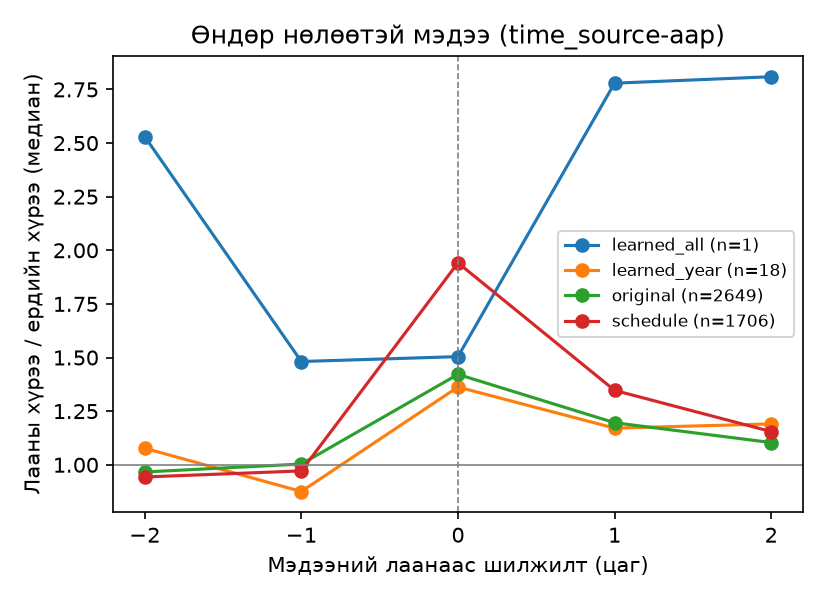
\includegraphics[width=0.8\textwidth]{Pictures/news_timing_check.png}
\caption{Мэдээний цагийн шалгалт: мэдээний лаанаас $\pm2$ цагийн дундаж хүрээ}
\label{fig:timing}
\end{figure}

\section{Мэдээний нөлөө}

\subsection{Нөлөөний түвшин}
ForexFactory мэдээ бүрийг шинжээчдийн үнэлгээгээр бага, дунд, өндөр нөлөөтэй гэж ангилдаг. Энэ ангиллыг өгөгдлөөр
шалгасан (\tref{tab:impact}).

\begin{table}[H]
\centering
\caption{Мэдээний нөлөөний түвшин ба бодит хөдөлгөөн (USD/EUR, 2015--2025)}
\label{tab:impact}
\small
\begin{tabular}{lrrrr}
\toprule
\textbf{Түвшин} & \textbf{Мэдээ} & \textbf{60 мин хүрээ, пип} & \textbf{Ердийн цагаас} & \textbf{2 дахинаас их} \\
\midrule
Бага (Low)    & 9\,244 & 16.9 & $\times$1.02 & 6.9\% \\
Дунд (Medium) & 3\,278 & 19.8 & $\times$1.07 & 7.8\% \\
Өндөр (High)  & 2\,557 & 28.5 & $\times$1.41 & 29.7\% \\
\bottomrule
\end{tabular}
\end{table}

Бага, дунд нөлөөтэй мэдээний үед ханш ердийнхөөсөө бараг ялгаагүй хөдөлдөг. Өндөр нөлөөтэй мэдээний үед дунджаар
1.4 дахин, FOMC-ийн үед 5 дахин, ECB-ийн хүүгийн шийдвэрийн үед 2.8 дахин, NFP-ийн үед 2.5 дахин том хөдөлдөг.
Харин газрын тосны нөөцийн мэдээ өндөр нөлөөтэй гэж ангилагдсан ч EUR/USD-д нөлөөгүй ($\times$1.04).

\textbf{Шийдвэр:} загварт зөвхөн өндөр нөлөөтэй мэдээг ашиглана. Мэдээний төрөл бүрийн түүхэн нөлөөг тусад нь шинж
болгоно.

\subsection{Мэдээний нөлөө хэр удаан үргэлжилдэг вэ}
Surprise-ийн чиглэл мэдээ гарсны дараах эхний 5 минутын хөдөлгөөний чиглэлтэй 1\,043 үйл явдлын 69.4\%-д таарсан
(\fref{fig:news}). Энэ нь мэдээний цаг, утга зөв гэдгийн хамгийн хүчтэй нотолгоо мөн. Хэрэв цаг эсвэл утга буруу байсан
бол таарц 50\% гарах байсан.

Гэвч хөдөлгөөний 80\% орчим нь мэдээ гарснаас хойш \emph{эхний 1 минутад} болдог. Эхний 5 минутын дараах чиглэл
санамсаргүй (~50\%) байна. Тохиолдлын ~30\%-д чиглэл таараагүй шалтгааны гуравны хоёр нь зах зээл хариу үзүүлээгүй,
нэг цагт эсрэг чиглэлтэй мэдээ гарсан, эсвэл тухайн мэдээ EUR/USD-д хамааралгүй байсанд оршино.

\begin{figure}[H]
\centering
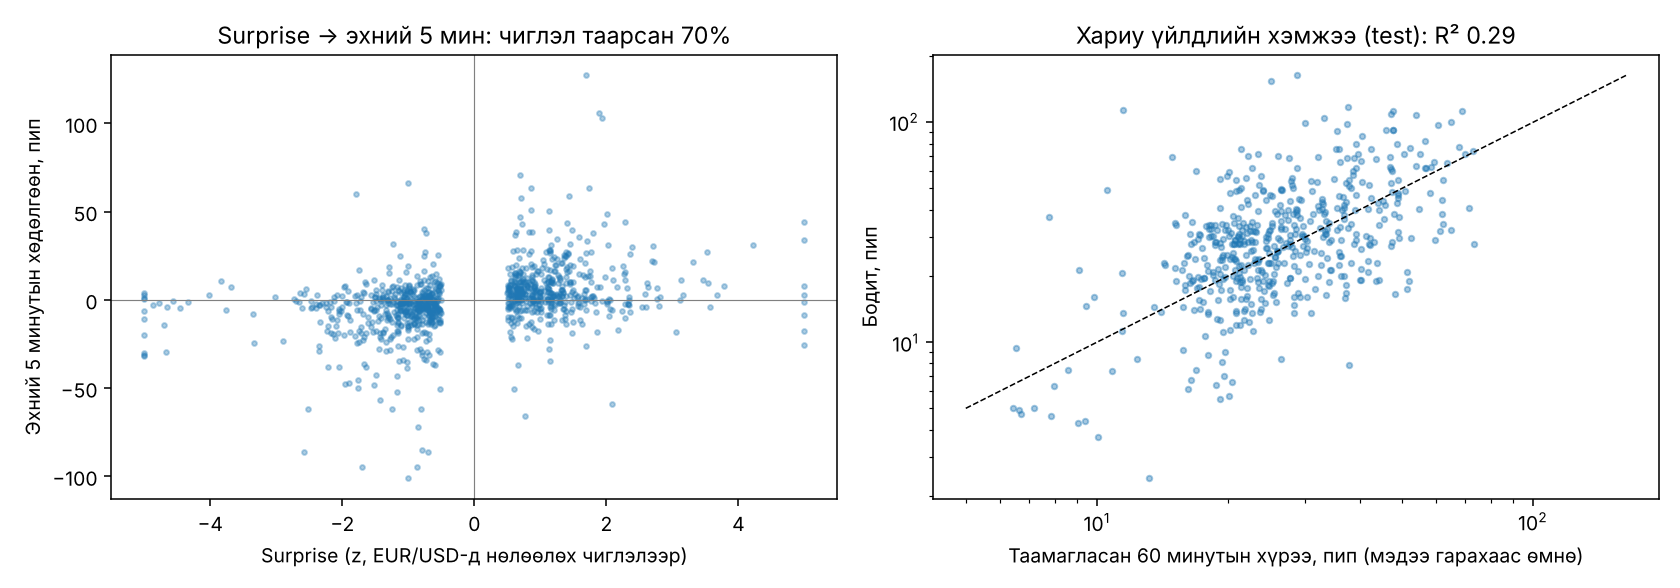
\includegraphics[width=\textwidth]{Pictures/news_analysis.png}
\caption{Мэдээний surprise ба эхний 5 минутын хөдөлгөөний хамаарал}
\label{fig:news}
\end{figure}

\textbf{Дүгнэлт:} мэдээ гарсны дараа чиглэлийг ашиглах боломж маш богино. Харин мэдээ гарахаас \emph{өмнө} хөдөлгөөн
хэр том байхыг мэдээний төрлөөр урьдчилан хэлж болно. Иймд загварт мэдээний бодит утгаас илүүтэй мэдээний хуваарь
(дараагийн мэдээ хүртэлх хугацаа, мэдээний төрөл) чухал байх магадлалтай. Үүнийг 12-р сард шалгана.
